\documentclass[12pt]{article}
% Reduce excessive hyphenation https://stackoverflow.com/a/65156105
\tolerance=9999
\emergencystretch=10pt
\hyphenpenalty=10000
\exhyphenpenalty=100

\usepackage[
top=1cm,
bottom=1cm,
left=1cm,
right=1cm,
headsep=6pt,
headheight=17pt, % as per the warning by fancyhdr
includehead,
heightrounded, % to avoid spurious underfull messages
]{geometry}
\usepackage{hyperref}           % clickable links
\hypersetup{colorlinks=true,citecolor=blue,linkcolor=blue,urlcolor=blue}
\urlstyle{rm}
\usepackage[nameinlink]{cleveref}
\newcounter{cls}
\newcommand{\labelcls}[1]{\refstepcounter{cls}\thecls\label{#1}}
\crefalias{cls}{assgn}
\crefname{assgn}{assignment}{assignments}
\usepackage{fancyhdr}
\newcommand{\smallerfont}{\fontsize{11}{13}\selectfont}
\fancypagestyle{plain}{%
  \fancyhf{}                      % Clear header and footer fields.
  \fancyhead[l]{\smallerfont{}Spring 2026}
  \fancyhead[c]{\smallerfont{}Syllabus: MSMI 3450: GPUs for Massively Parallel Mechanistic Modeling (3~credits)}
  \fancyhead[r]{\smallerfont{}Page \thepage{} of~\pageref*{mylastpage}}}
\pagestyle{plain}
\usepackage{graphicx}
\graphicspath{{img/}}
\usepackage{sectsty}            % sectionfont
\sectionfont{\fontsize{12}{15}\selectfont}
\usepackage{soul}
\usepackage[
abbreviate=true,
bibencoding=utf8,
minnames=2,
maxbibnames=99,
sorting=none,
style=vancouver,
citestyle=numeric-comp
]{biblatex}
% The vancouver citation style is based on NLM per
% https://tex.stackexchange.com/a/371433
\addbibresource{references.bib}
\usepackage{upgreek}                % \upalpha
% Highlight author.
\renewcommand*{\mkbibnamegiven}[1]{%
  \ifitemannotation{highlight}{\textbf{\color{red} #1}}{#1}}
\renewcommand*{\mkbibnamefamily}[1]{%
  \ifitemannotation{highlight}{\textbf{\color{red} #1}}{#1}}
% Bibliography text size.
\renewcommand*{\bibfont}{\footnotesize}
\usepackage{tabularx}           % Table with X variable width wrapping column.
\usepackage{supertabular}       % Table that breaks across pages.
\usepackage{booktabs}           % {top,mid,bottom}rule
\usepackage[table]{xcolor}      % \rowcolor
\usepackage{callouts-box}
\usepackage{datetime2}
\DTMsavedate{class-begin}{2026-01-12}
\DTMsavedate{class-drop}{2026-01-23}
\DTMsavedate{break-begin}{2026-03-09}
\DTMsavedate{break-end}{2026-03-13}
\DTMsavedate{exam-conflict}{2026-03-16}
\DTMsavedate{class-withdraw}{2026-03-20}
\DTMsavedate{class-end}{2026-04-24}
\DTMsavedate{exam-begin-grad}{2026-04-25}
\DTMsavedate{exam-end-grad}{2026-05-02}
\DTMsavedate{exam-begin-ug}{2026-04-26}
\DTMsavedate{exam-end-ug}{2026-05-01}
\DTMsavedate{grades-due}{2026-05-05}
\usepackage{clipboard}
\usepackage{tikz}
\usetikzlibrary{mindmap}

\begin{document}

% https://poorvucenter.yale.edu/teaching/teaching-resource-library/syllabus-design

% https://hpcic.llnl.gov/tutorials/2025-hpc-tutorials

\begin{description}
\item[Instructor] Pariksheet Nanda, PhD \quad %
  \href{mailto:pan79@pitt.edu}{pan79@pitt.edu} \quad %
  The Assembly \#3099 \quad %
  Mo, Tu 13:00--15:00
\end{description}

\section{Course description}

Graphical Processing Units (GPUs) %
are not just for artificial intelligence (AI) or %
video games!
%
\ul{GPUs now power the worlds fastest supercomputers %
to solve the most computationally difficult, %
mechanistic scientific problems} in %
physics, %
chemistry, %
biology, %
material sciences, %
energy, %
earth and space sciences, %
national security, %
data analytics, and %
optimization.
%
An 8~year, \$1.8~billion effort %
called the Exascale Computing Project %
involving 2,800 scientists and engineers %
recently finished modernizing %
the underlying scientific numerical software %
to efficiently use this new generation of machines %
at more than a billion, billion floating point calculations per second %
referred to as exaflops.
%
While the National Science Foundation (NSF) NAIRR %
and the computing facilities themselves directly grant %
U.S. institutional and industry researchers like you %
\ul{to use these machines for your research projects at no cost, %
you have to do the work showing that %
your computations efficiently use %
multiple GPUs across many computer servers, %
thus scaling to solve large computational problems}.
%
This class will teach you %
computational skills to program for data parallel architecture, %
statistical techniques to tune your model to match heterogeneous datasets, %
testing and feedback %
to regularly verify and improve your software quality, %
and you will solve a real-world research problem with your own faculty mentor.

This elective course is intended for %
graduates trainees, %
ideally in their first or second year from admission %
to benefit from applying the class skills %
toward their thesis work.
%
\ul{All trainees %
must e-mail the instructor a letter of support from a faculty mentor %
before the course begins} %
for the instructor to help scope the capstone project %
and to group learners in complementary research areas together.
%
This course does not directly focus on AI tools %
but instead focuses on high performance computing (HPC) tools %
and HPC numerical libraries %
that can be instrumented for hardware performance analysis;
trainees interested in AI-coupled research applications %
will benefit by being able to run their workloads %
on the same set of GPU accelerators.

\noindent
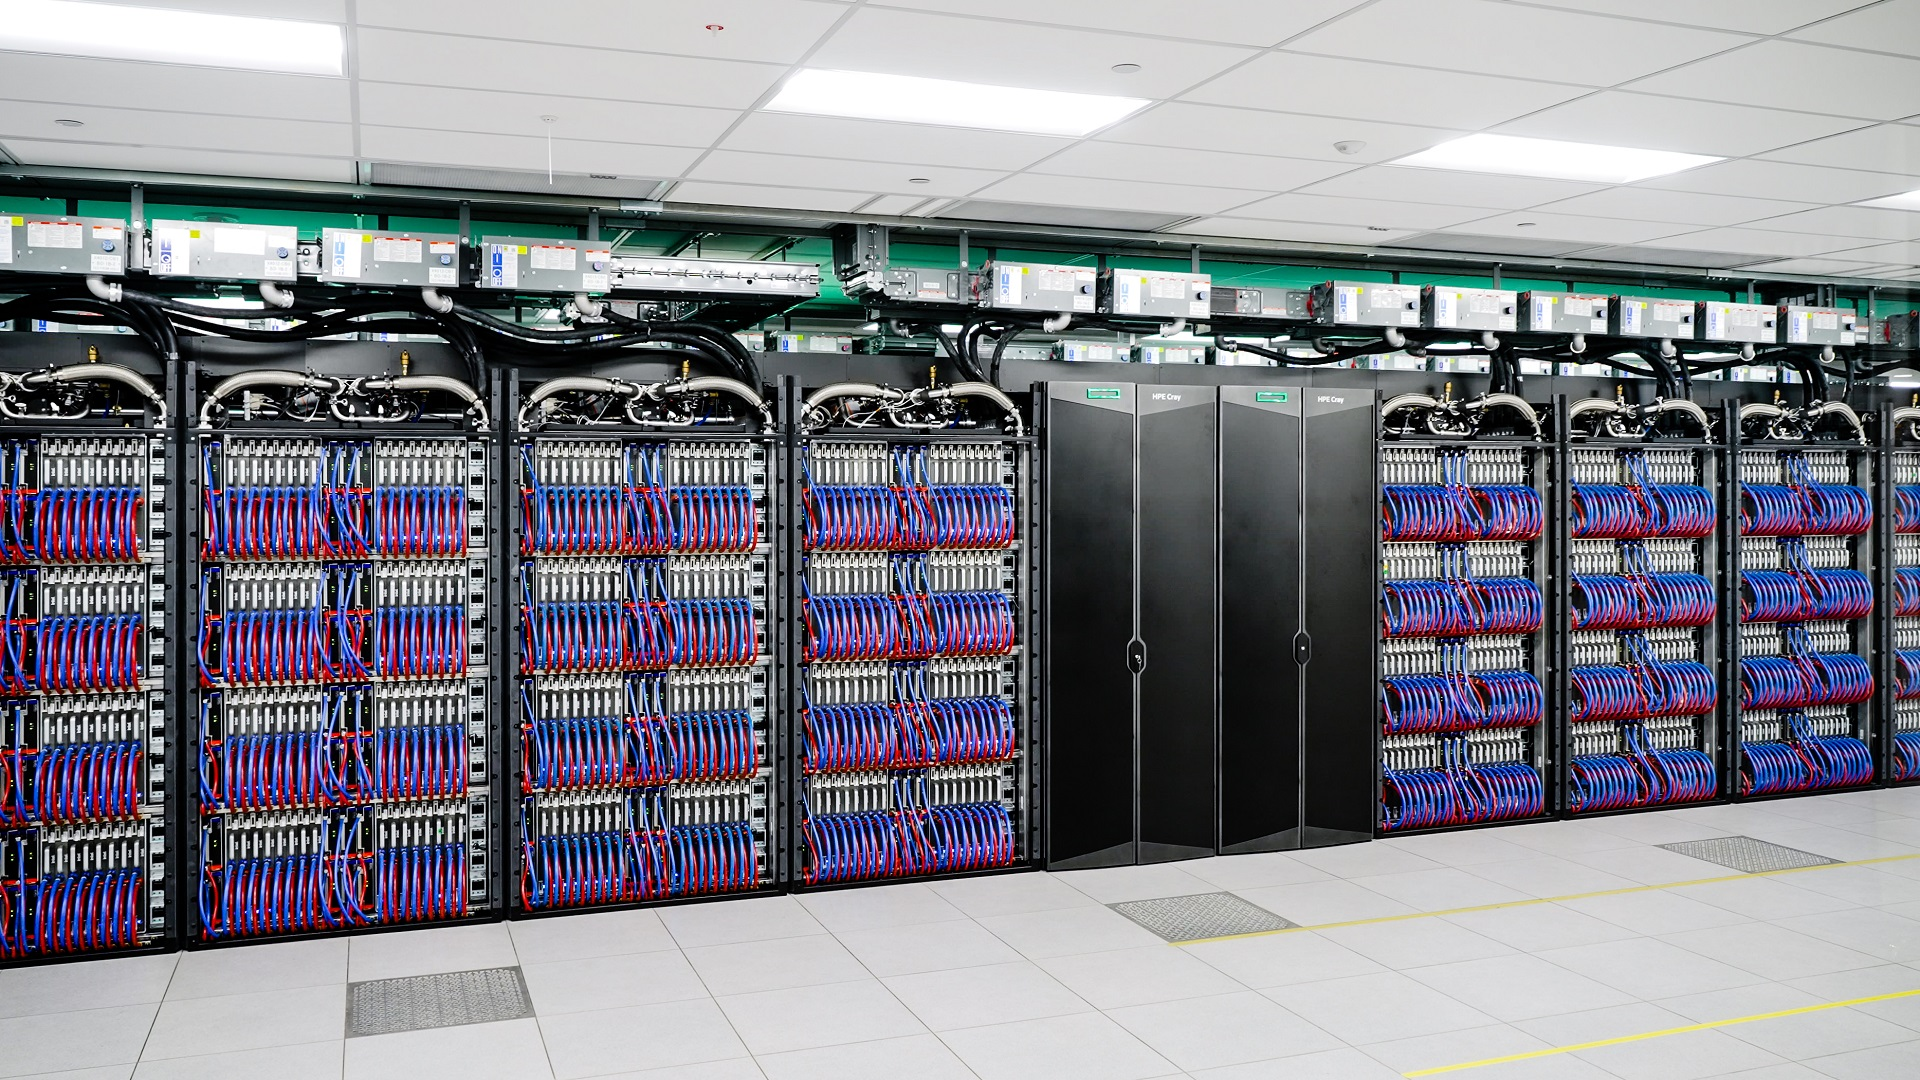
\includegraphics[width=\linewidth]{1920x1080-Aurora hero image.jpg}
% https://www.anl.gov/sites/www/files/2024-05/1920x1080-Aurora hero image.jpg
Photo: The Aurora supercomputer at Argonne National Laboratory; %
rank 3 in the Top 500 List of June 2025.

\section{Course prerequisites}

\begin{itemize}
\item \ul{Familiarity with at least one %
  procedural computer programming language} %
  (such as C, C++, C\#, Fortran, Rust, Swift, %
  Python, R, Julia, GNU Octave, MATLAB, %
  Perl, Ruby, Java, Lisp, etc.)

  The class will use C++, Python, and %
  a small amount of Bash shell scripting.

  Don't worry about if you do not know any C++ or Python; %
  part of your performance engineering training %
  is to become a computer programming polyglot---%
  even professionals use resources like Learn X in Y minutes %
  to refresh themselves on how to do a computing task in a particular language.
\item \ul{Basic statistical knowledge} %
  of mean, median, standard deviation, and L2-norm.

  The class uses these statistical concepts to construct %
  summary functions for matching computational models with datasets; %
  they are also used in performance profiling tools.

  You will likely encounter more advanced statistics and mathematics %
  for your capstone project %
  and the instructor will do their best and work with your faculty mentor %
  to suggest supplementary books, review papers, or other resources %
  and adjust your class assignment commitments for you to pursue them.
\item \ul{A tentative topic for your capstone project}; %
  please suggest a tentative topic with a faculty mentor when %
  contacting the instructor for a permission number to join the course.
  %
  Note that %
  \ul{your topic is expected to change at least somewhat %
  during the first 3~weeks of the course}, %
  therefore your topic is not ``set in stone'' until \Cref{a-gpu}-capstone %
  due at the $4^{\mathrm{th}}$ week of the course.

  The course may accommodate advanced undergraduates %
  without research faculty mentors %
  or existing research projects; %
  a list of suggested projects are provided in %
  appendix \Cref{sec:projects} Projects for advanced undergraduates.
  %
  In this case, %
  the capstone project would count toward a subsequent application to %
  summer NSF research experiences for undergraduates (REU) %
  and/or collaborations with research core-facility staff or faculty.
\end{itemize}

\section{Required resources}

\begin{itemize}
\item \ul{Laptop computer to use in class} running an operating system %
  supported for scientific processing and visualization software %
  such as GNU/Linux, macOS, or Windows %
  (namely, ChromeBooks, tablets, and smartphones would likely not be suitable).

  Typically, %
  GNU/Linux is best supported %
  in computationally-intensive scientific computing %
  and immersing yourself using that as your everyday operating system %
  will support a career in this field; %
  several commercial vendors sell GNU/Linux laptops\footnote{%
  % US-based - only GNU/Linux.
  System76, ThinkPenguin, Purism, %
  % US-based - optional GNU/Linux.
  Framework, Malibal, %
  % International.
  NovaCustom, Tuxedo Computers, StarLabs, Slimbook, %
  % Refurbished.
  Technoethical, Vikings, Libiquity, etc.}.
  %
  For the purposes of this class, %
  a laptop GPU with compute capability\footnote{%
  Intel Xe (in Intel Arc GPUs), AMD ROCm, and Nvidia CUDA.} %
  would allow you to develop and test code locally %
  with more control than testing on remote machines.
\end{itemize}

\noindent
No software installation is necessary before the course begins.

\section{Assessment}

Theoretical portions of assignments will be graded using Canvas, %
however the majority of this course %
consists of practical code exercises %
that will be submitted using the git version control system.
%
These exercises will be tested and graded using %
a custom GitLab-CI runners and repositories %
setup by the instructor, %
necessary for the complex multi-node and multi-GPU environments.
%
There are no planned examinations %
because the capstone project %
sufficiently assesses coursework proficiency.

\section{Learning objectives}

\begin{enumerate}
\item Write \ul{per-node vectorized} CPU and GPU code.
  %
  Analyze per-node efficiency using assembly instructions, %
  memory hierarchy, FLOP-memory bandwidth, and %
  compare against algorithmic complexity.
\item Architect \ul{multi-node distributed} software.
  %
  Analyze multi-node bottlenecks using SLURM statistics, %
  Darshan, and HPCToolKit.
\item Fit compute-intensive scientific software %
  to \ul{heterogeneous datasets} %
  using distributed, parallelizable samplers.
\item Develop scientific code specific %
  \ul{unit tests and performance regression tests} %
  for sustainable software.
  %
  Describe and document scientific codes at appropriate levels.
\item Communicate with peers to give \ul{constructive code criticism} %
  using issue trackers, git merge/pull requests, and review comments.
\item Apply the above skills in developing a \ul{capstone portfolio project}.
  %
  Write an NSF ACCESS style report %
  using a scaling study to justify a request for computational resources.
  %
  Oral presentations of capstone progress and final outcome.
\end{enumerate}

\noindent
Corresponding \ul{learning goals %
are listed at the end of each class} %
in the table in \Cref{sec:course-schedule} Course schedule.

\section{Course topic categories}

The topics covered in this course %
can be thought of as being the following categories of %
the capstone project,
performance optimization, %
software development, %
domain science, and %
cluster administration:

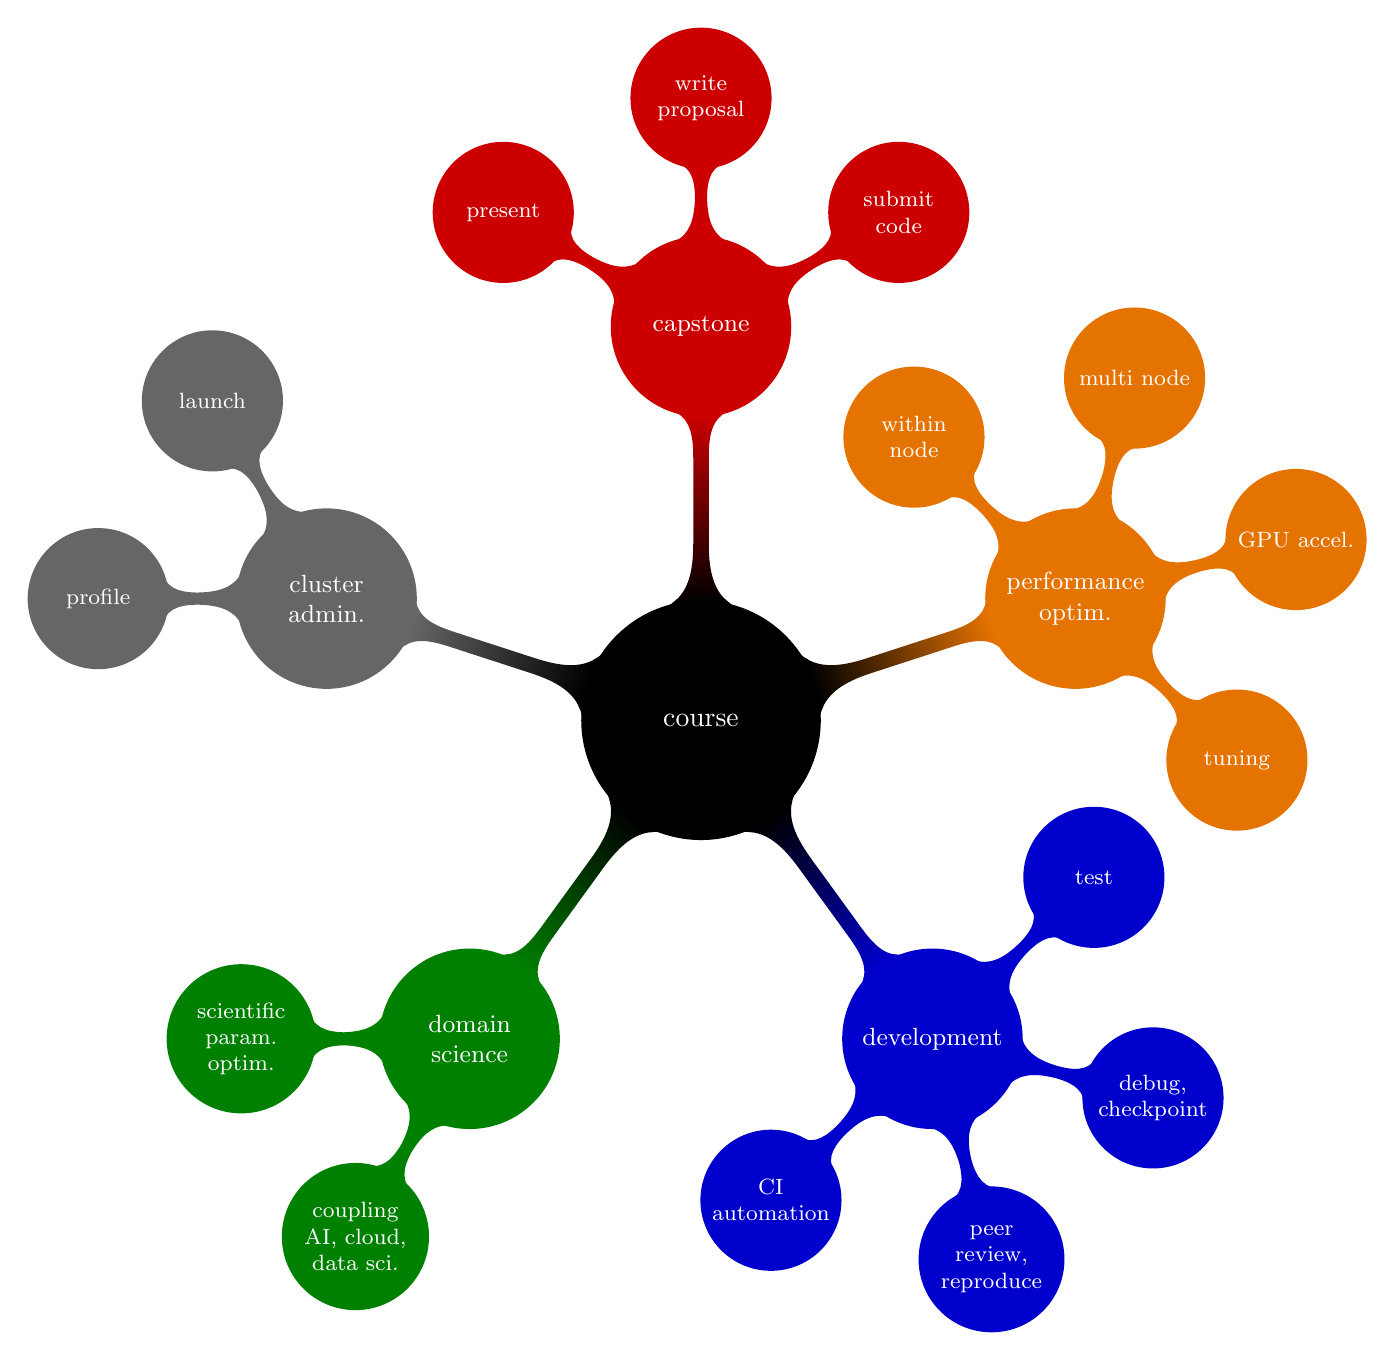
\begin{tikzpicture}[
  root concept/.style={
    minimum size=3cm,
  }
  ]
  \path [mindmap]
  node [concept, concept color=black, text=white] {course}
  child [grow=90, concept color=red!80!black, text=white] {
    node [concept] {capstone}
    [clockwise from=150]
    child { node [concept] {present} }
    child { node [concept] {write proposal} }
    child { node [concept] {submit code} }
  }
  child [grow=18, concept color=orange!90!black, text=white] {
    node [concept] {performance optim.}
    [clockwise from=135]
    child { node [concept] {within node} }
    child { node [concept] {multi node} }
    child { node [concept] {GPU accel.} }
    child { node [concept] {tuning} }
  }
  child [grow=306, concept color=blue!80!black, text=white] {
    node [concept] {development}
    [clockwise from=45]
    child { node [concept] {test} }
    child { node [concept] {debug, checkpoint} }
    child { node [concept] {peer review, reproduce} }
    child { node [concept] {CI automation} }
  }
  child [grow=234, concept color=green!50!black, text=white] {
    node [concept] {domain science}
    [counterclockwise from=180]
    child { node [concept] {scientific param. optim.} }
    child { node [concept] {coupling AI,~cloud, data sci.} }
  }
  child [grow=162, concept color=black!60, text=white] {
    node [concept] {cluster admin.}
    [counterclockwise from=120]
    child { node [concept] {launch} }
    child { node [concept] {profile} }
  };
\end{tikzpicture}

\section{Course schedule}%
\label{sec:course-schedule}

\noindent
Classes are on Wednesdays at 13:00--14:50.
%
Broadly speaking, the schedule is divided into two halves:
\begin{enumerate}
\item Intensive instruction of critical skills %
  to support you working on your capstone project, and
\item Advanced topics that may or may not support your capstone project, %
  but that hopefully expand your capabilities.
  %
  You will also present regular progress reports on your capstone project.
\end{enumerate}

\newcommand{\myheader}{%
  Date & Topic, assignment, goal & Assignment(s) due on this date}
\tablefirsthead{
  \toprule
  \myheader \\
  \midrule}
\tablehead{
  \multicolumn{3}{c}{Table continued from previous page} \\
  \toprule
  \myheader \\
  \midrule}
\tabletail{
  \midrule
  \multicolumn{3}{c}{Table continued on next page} \\}
\tablelasttail{\bottomrule}
% Table row spacing
\renewcommand{\arraystretch}{2}
% Use primitive for text width, because widthof does not work inside the table
% header:  https://tex.stackexchange.com/a/18577
\newdimen\widthdate
\setbox0=\hbox{4444-44-44}
\widthdate=\wd0
\noindent
\begin{mpsupertabular}{%
    % Dimensions from https://tex.stackexchange.com/a/62718
  p{\dimexpr \widthdate} | %
  p{\dimexpr .695\linewidth-3\tabcolsep-.5\widthdate} | %
  p{\dimexpr .305\linewidth-3\tabcolsep-.5\widthdate}}
  \DTMdate{2026-01-14}
  & \textbf{Topic~\labelcls{a-node}: Strategies for %
    within-node vectorization, %
    caching, %
    memory bandwidth, and %
    I/O}.

    \vspace{.5\baselineskip}
    Assignment~\labelcref{a-node}: %
    Exercises vectorizing Python code, %
    inspecting C assembler CPU vectorized instructions, %
    creating roofline plots to inspect CPU-memory, %
    hwloc to inspect memory CPU hierarchy.

    \vspace{.5\baselineskip}
    Goal \labelcref{a-node}: %
    Learn how to check and write code for efficient low-level execution; %
    practice submitting assignments using Git.
  & ---\\
  \DTMdate{2026-01-21}
  & \textbf{Topic~\labelcls{a-clust}: %
    Strategies for task distribution and multi-node cluster scaling}.

    \vspace{.5\baselineskip}
    Assignment~\labelcref{a-clust}: %
    Exercises with C, TaskWorks\footnote{%
    \url{https://github.com/hpc-io/taskworks}}, %
    Spack, MPI, and SLURM.\@

    \vspace{.5\baselineskip}
    Goal~\labelcref{a-clust}: Accommodate blocking operations (e.g. I/O) %
    using batching and threading.
  & \Cref{a-node}\\
  \rowcolor{gray!20}
  \DTMusedate{class-drop}
  & \multicolumn{2}{l}{Deadline for advanced undergraduates %
    to submit their research staff / faculty letter of support.} \\
  \rowcolor{gray!20}
  & \multicolumn{2}{l}{Deadline to drop classes.} \\
  \DTMdate{2026-01-28}
  & \textbf{Topic~\labelcls{a-gpu}: %
    Introduction to data parallel programming for GPUs}.

    \vspace{.5\baselineskip}
    Assignment~\labelcref{a-gpu}: %
    Exercises with C++ SYCL and Kokkos %
    to fill in the blanks of partially completed programs.

    Assignment~\labelcref{a-gpu}-capstone: %
    Outline an informal bullet list of goals and objectives %
    to create a minimum viable product of your scientific code %
    through the remainder of the semester.

    \vspace{.5\baselineskip}
    Goal~\labelcref{a-gpu}: Implement algorithms %
    using heterogeneous computing frameworks.

    Goal 3-capstone: %
    You now have sufficient background %
    to begin planning your capstone assignment.
  & \Cref{a-clust}\\
  \DTMdate{2026-02-04}
  & \textbf{Topic~\labelcls{a-fit}: Gradient based and %
    pseudo-likelihood based %
    parallel parameter fitting}.

    \vspace{.5\baselineskip}
    Assignment~\labelcref{a-fit}: Exercises with %
    distributed gradient-based parameter fitting, and %
    pyABC ABC-SMC.\@

    Assignment~\labelcref{a-fit}-capstone: %
    Import your datasets and %
    choose a gradient-based or gradient-free method %
    to sample parameters your solver %
    that best match your datasets.

    \vspace{.5\baselineskip}
    Goal~\labelcref{a-fit}: Apply statistical summaries %
    to match solver outputs with datasets %
    using gradient-based and gradient-free sampling techniques.

    Goal~\labelcref{a-fit}-capstone: %
    Apply your domain knowledge %
    to appropriately match your datasets to your solver outputs.
  & \Cref{a-gpu},

    \Cref{a-gpu}-capstone\\
  \DTMdate{2026-02-11}
  & \textbf{Topic~\labelcls{a-tune}: %
    Introduction to distributed performance tuning}.

    \vspace{.5\baselineskip}
    Assignment~\labelcref{a-tune}: Exercises with Darashan, Drishti\footnote{%
    \url{https://github.com/hpc-io/drishti-io}}, and %
    HPCtoolkit

    Assignment~\labelcref{a-tune}-capstone: %
    Literature review of software similar to yours %
    and how you intend to make yours different.

    \vspace{.5\baselineskip}
    Goal~\labelcref{a-tune}: Synthesize previous concepts from Topics 1--3 %
    to critically assess and improve program performance.

    Goal~\labelcref{a-tune}-capstone: %
    You will revisit distributed performance tuning as needed %
    during the remainder of the semester; %
    instead focus your efforts into why makes your project unique %
    by reviewing prior art.
  & \Cref{a-fit},

  \Cref{a-fit}-capstone\\
  \DTMdate{2026-02-18}
  & \textbf{Topic~\labelcls{a-test}: %
    Automated unit testing, performance regression testing, and test coverage}.

    \vspace{.5\baselineskip}
    Assignment~\labelcref{a-test}: Exercise with professor and pairing

    \vspace{.5\baselineskip}
    Goal~\labelcref{a-test}: [\ldots]
  & \Cref{a-tune},

  \Cref{a-tune}-capstone\\
  \DTMdate{2026-02-25}
  & \textbf{Topic~\labelcls{a-rev}: %
    Practicing stress-free peer review of code and %
    writing various types of documentation}.

    \vspace{.5\baselineskip}
    Assignment~\labelcref{a-rev}: Exercise with professor and pairing

    \vspace{.5\baselineskip}
    Goal~\labelcref{a-rev}: [\ldots]
  & \Cref{a-test},

  \Cref{a-test}-capstone\\
  \DTMdate{2026-03-04}
  & \textbf{Topic~\labelcls{a-next}: Continuous integration systems, %
    git hooks, etc.\@ for testing and documentation}.
  & \Cref{a-rev},

  \Cref{a-rev}-capstone\\
  \rowcolor{gray!20}
  \multicolumn{3}{c}{Enjoy your spring break! %
  No assignments and no classes %
  \DTMusedate{break-begin} through %
  \DTMusedate{break-end}.}\\
  \DTMdate{2026-03-18}
  & \textbf{Topic~\labelcls{a-ckpt-dbg}: Checkpointing and parallel debugging}.

    \vspace{.5\baselineskip}
    Assignment~\labelcref{a-ckpt-dbg}: [\ldots]

    \vspace{.5\baselineskip}
    Goal~\labelcref{a-ckpt-dbg}: [\ldots]
  & ---\\
  \DTMdate{2026-03-25}
  & \textbf{Topic~\labelcls{a-beyond-hpc}: Coupling HPC paradigms %
    with data science, AI, and cloud environments}.

    \vspace{.5\baselineskip}
    Assignment~\labelcref{a-beyond-hpc}:
    Summarize the key concepts of chapters 4 and 8 of ISBN 978-3-031-78698-3; %
    in no more than a single page.

    \vspace{.5\baselineskip}
    Goal~\labelcref{a-beyond-hpc}: [\ldots]

    \vspace{.5\baselineskip}
    Assignment~\labelcref{a-beyond-hpc}-capstone: %
    Assess possible extensions to your capstone project %
    using components of AI, big data, or cloud applications %
    and specialized hardware needs %
    by connecting the concepts from each of the two articles, %
    your domain science, and %
    to what extent we discussed these concepts so far in the class.

    \vspace{.5\baselineskip}
    Goal~\labelcref{a-beyond-hpc}-capstone: [\ldots]
  & \Cref{a-ckpt-dbg},

  \Cref{a-ckpt-dbg}-capstone\\
  \DTMdate{2026-04-01}
  & \textbf{Topic~\labelcls{a-self-host}: Collaboratively launch %
    your own HPC cluster}.

    \vspace{.5\baselineskip}
    Assignment~\labelcref{a-self-host}: [\ldots]

    \vspace{.5\baselineskip}
    Goal~\labelcref{a-self-host}: [\ldots]

    \vspace{.5\baselineskip}
    Assignment~\labelcref{a-self-host}-capstone: [\ldots]

    \vspace{.5\baselineskip}
    Goal~\labelcref{a-self-host}-capstone: [\ldots]
  & \Cref{a-beyond-hpc},

  \Cref{a-beyond-hpc}-capstone\\
  \DTMdate{2026-04-08}
  & \textbf{Topic~\labelcls{a-self-bench}: Benchmark and troubleshoot %
    your HPC cluster}.

    \vspace{.5\baselineskip}
    Assignment~\labelcref{a-pres-1}-capstone (group 1) %
    \Copy{assignment-last-presentation}{%
    15 minute final presentations %
    summarizing program architecture, %
    critical benchmarks including weak and strong scaling, %
    overview of semester timeline %
    including incorporation of course materials and practices, %
    and future directions.}

    \vspace{.5\baselineskip}
    Goal~\labelcref{a-pres-1}-capstone (group 1): %
    \Copy{goal-last-presentation}{%
    Self-assess progress and %
    prepare preliminary data for grant application.}
  & \Cref{a-self-host},

  \Cref{a-self-host}-capstone\\
  \DTMdate{2026-04-15}
  & \textbf{Topic~\labelcls{a-pres-1}: Presentations of capstone project %
    (group 1)}.

    \vspace{.5\baselineskip}
    Assignment~Last-capstone (group 1): %
    \Copy{assignment-last-submit}{%
    Write either an NSF ACCESS Discover application %
    or equivalent supporting grant section in your discipline %
    using material from your final presentation %
    summarizing overall scientific value, %
    code architecture, %
    critical benchmarks including weak and strong scaling, %
    referencing software engineering practices and sustainability %
    where possible, %
    expected impact and future directions.}

    \vspace{.5\baselineskip}
    Goal Last-capstone (group 1): Synthesize your analysis %
    \Copy{goal-last-submit}{%
    Synthesize the analyses from your final presentation %
    into a formal written allocation application or domain grant; %
    the written document must address all criticism from the presentation %
    by the instructor and from classroom peers that the instructor %
    will summarize for you after your presentation.}

    \vspace{.5\baselineskip}
    Assignment~\labelcref{a-pres-2}-capstone (group 2): %
    \Paste{assignment-last-presentation}

    \vspace{.5\baselineskip}
    Goal~\labelcref{a-pres-2}-capstone (group 2): %
    \Paste{goal-last-presentation}
  & \Cref{a-pres-1}-capstone (group 1) \\
  \DTMdate{2026-04-22}
  & \textbf{Topic~\labelcls{a-pres-2}: Presentations of capstone project %
    (group 2)}.

    Assignment~Last-capstone (group 2): %
    \Paste{assignment-last-submit}

    \vspace{.5\baselineskip}
    Goal Last-capstone (group 2): %
    \Paste{goal-last-submit}
  & \Cref{a-pres-2}-capstone (group 2) \\
  \DTMusedate{exam-end-ug}
  & \textbf{Deadline to turn in capstone project with grant application.}
  & Capstone project code and %
    written allocation or grant application %
    (groups 1 and 2) \\
  \rowcolor{gray!20}
  \DTMusedate{grades-due}
  & \multicolumn{2}{l}{Grades due.} \\
\end{mpsupertabular}

\begin{notebox}
  The sections below contain language provided by the university.
  %
  Inapplicable text for this course is formatted with strike-through marks %
  with explanatory footnotes.
\end{notebox}

\section{Academic integrity}

Students in this course %
will be expected to comply with %
the University of Pittsburgh's %
Policy on Academic Integrity%
\footnote{\url{https://www.provost.pitt.edu/info/ai1.html}}.
%
Any student suspected of violating this obligation %
for any reason during the semester %
will be required to participate in the procedural process, %
initiated at the instructor level, %
as outlined in the University Guidelines on Academic Integrity.
%
This may include, %
but is not limited to, %
the confiscation of the examination %
of any individual suspected of violating University Policy.
%
\st{Furthermore, %
no student may bring any unauthorized materials to an exam, %
including dictionaries and programmable calculators.}\footnote{%
This facet of the university policy does not apply to this class.}

To learn more about Academic Integrity, %
visit the Academic Integrity Guide%
\footnote{\url{http://pitt.libguides.com/academicintegrity/}} %
for an overview of the topic.
%
For hands-on practice, %
complete the Academic Integrity Modules%
\footnote{\url{http://pitt.libguides.com/academicintegrity/plagiarism}}.

\section{Disability services}

If you have a disability %
for which you are or may be requesting an accommodation, %
you are encouraged to contact %
both your instructor and Disability Resources and Services (DRS)%
\footnote{\url{https://www.studentaffairs.pitt.edu/drs/}}, %
140 William Pitt Union, %
(412)~648-7890, %
\href{mailto:drsrecep@pitt.edu}{drsrecep@pitt.edu}, %
(412)~228-5347 for P3 ASL users, %
as early as possible in the term.
%
DRS will verify your disability %
and determine reasonable accommodations for this course.

\label{mylastpage}              % chktex 24
\newpage
\appendix
\setcounter{page}{1}
\renewcommand{\thepage}{\arabic{page}}
\fancyhead[c]{References}
\fancyhead[r]{Appendix Page \thepage{} of~\pageref*{mylastappendixpage}}

\section{Projects for advanced undergraduates}
\label{sec:projects}



\printbibliography[heading=none]{}%
\label{mylastappendixpage}

\end{document}
